\subsubsection{Vorteile von Polycarbonat gegenüber anderen Materialien}

Polycarbonat wurde 1953 von dem, bei der Firma Bayer angestellten, Chemiker
Hermann Schnell entdeckt. Der neue Kunststoff wurde später unter dem Namen
Makrolon\textsuperscript{\textregistered} vermarktet.

Nachdem seine ersten CD-Prototypen hergestellt hat, suchte man nach
Trägermaterial, welches für die Massenproduktion mittels des
Spritzgussverfahrens geeignet ist. Hierfür ist Polycarbonat nahezu perfekt. Die
niedriege Viskosität ermöglicht eine fehlerfreie übertragung der Pitstruktur von
der Matrize auf die Polycarbonatscheibe. Hohe Transparenz und ein konstater
Brechungsindex\footnote{Verhältnis der Lichtgeschwindigkeit und der
Ausbreitungsgeschwindigkeit von Licht im untersuchten Material} erlauben ein
unabgeschwächtes Durchdringen des Laserstrahls durch das Trägermaterial. Eine
hohe Erweichungstemperatur\footnote{ca. 149°C} und Resistenz gegenüber
physikalischen Belastungen machen Polycarbonat ebenfalls alltagstauglich.

Die ABB.VERGLEICH vergleicht Polycarbonat(PC) und Polymethylmethacrylat(PMMA) im
Bezug auf Eigenschaften, die für die Herstellung und Benutzung der CD von
Vorteil sind. Die Eignung nimmt in den jeweiligen Punkten von innen nach außen
zu. PMMA schneidet in fast allen Punkten mit Bestnote ab. Jedoch machen ein
insgesamt mittelmäßiges Abschneiden von PC und bessere Eigenschaften in den
Kategorien Wärmeformbeständigkeit und geringe Wasseraufnahme als
Polymethylmethacrylat Polycarbonat zum bevorzugten Kunststoff für die
CD-Produktion.


\begin{figure}[h]
  \begin{center}
      \begin{minipage}[t]{\textwidth}
        \begin{center}
            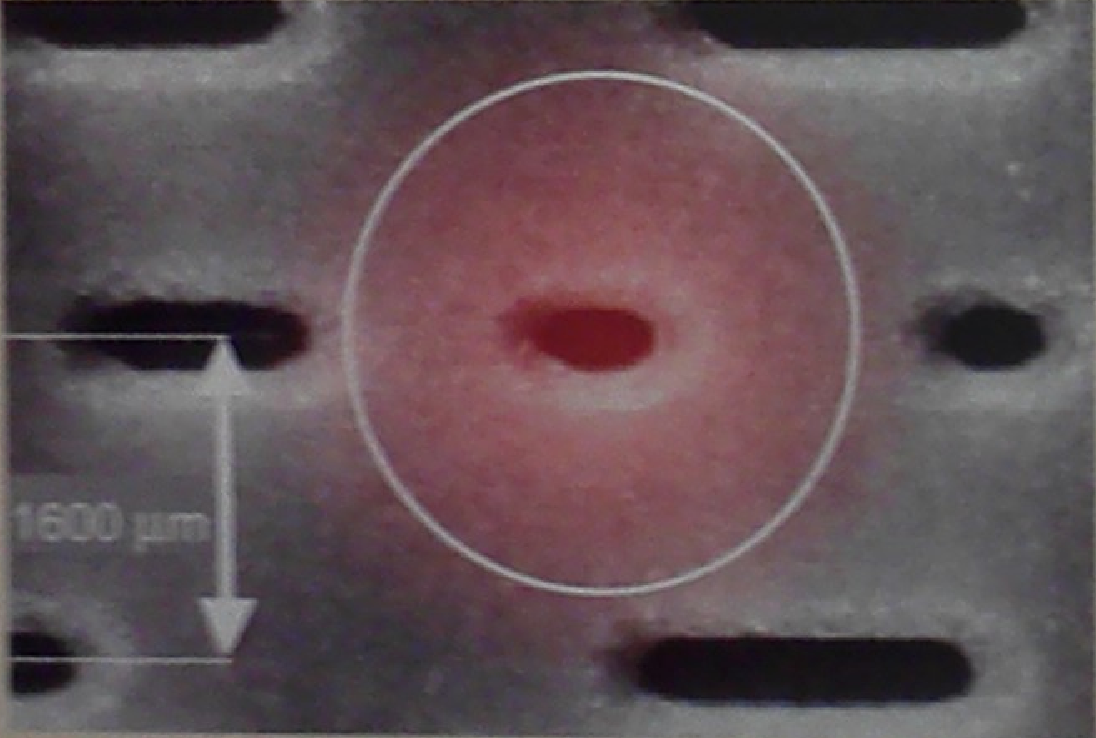
\includegraphics[height=0.1\textheight]{/home/i-bot/workspace/Seminararbeit/Bilder/Optische_Datentraeger_Die_Compact_Disc/Funktionsweise/remcd.png}
            \caption[ \newline Roth, Klaus: CD, DVD0 \& Co.: Die Chemie der schillernden Scheiben, in: Chemie in unserer Zeit (41/2007), S. 340]{Laserlicht auf einem \textit{pit} unter einem Rasterelektronenmikroskop}
            \label{fig:cdrem}
        \end{center}
      \end{minipage}
  \end{center}
\end{figure}
